 \documentclass{beamer}
%
% Choose how your presentation looks.
% For more themes, color themes and font themes, see:
% http://deic.uab.es/~iblanes/beamer_gallery/index_by_theme.html
%
\mode<presentation>
{
  \usetheme{Madrid}      % or try Darmstadt, Madrid, Warsaw, ...
  \usecolortheme{seahorse} % or try albatross, beaver, crane, ...
  \usefonttheme{serif}  % or try serif, structurebold, ...
  \setbeamertemplate{navigation symbols}{}
  \setbeamertemplate{caption}[numbered]
  \usepackage{amsmath}
  \usepackage{tcolorbox}
  \usepackage[export]{adjustbox}
  \tcbuselibrary{most}
  \usepackage{arydshln}
  \usepackage{tikz}
  \usetikzlibrary{plotmarks}
  \usepackage{pgfplots}
  \newcommand{\Ivec}[1]{\mbox{\boldmath $#1$}}
    \usepackage[normalem]{ulem}
    % \usepackage{tipa}
    \newcommand{\git}{\texttt{\textbf{git}}\xspace}
    \usepackage{listings}
} 


\definecolor{myblue}{RGB}{65,105,225} 
\definecolor{myorange}{RGB}{250,190,0}

\setbeamercolor{structure}{fg=white,bg=myorange}
\setbeamercolor*{palette primary}{fg=myblue,bg=myorange}
\setbeamercolor*{palette secondary}{fg=white,bg=myblue}
\setbeamercolor*{palette tertiary}{bg=myblue,fg=white}
\setbeamercolor*{palette quaternary}{fg=white,bg=myorange!50}

\setbeamercolor{frametitle}{fg=black!90!myblue}

\setbeamercolor{section in head/foot}{fg=white,bg=myblue}
\setbeamercolor{author in head/foot}{fg=black,bg=myorange}
\setbeamercolor{title in head/foot}{fg=white,bg=myblue}

\setbeamertemplate{navigation symbols}{}

\setbeamertemplate{itemize/enumerate body begin}{\large}
\setbeamertemplate{itemize/enumerate subbody begin}{\large}


\defbeamertemplate*{headline}{mytheme}
{%
  \begin{beamercolorbox}[ht=2.25ex,dp=3.75ex]{section in head/foot}
    \insertnavigation{\paperwidth}
  \end{beamercolorbox}%
}%

\defbeamertemplate*{footline}{mytheme}
{
  \leavevmode%
  \hbox{%
  \begin{beamercolorbox}[wd=.5\paperwidth,ht=2.25ex,dp=1ex,right]{author in head/foot}%
    \usebeamerfont{author in head/foot}\insertshortauthor\hspace*{2em}
  \end{beamercolorbox}%
  \begin{beamercolorbox}[wd=.5\paperwidth,ht=2.25ex,dp=1ex,left]{title in head/foot}%
    \usebeamerfont{title in head/foot}\hspace*{2em}\insertshortsubtitle\hspace*{2em}
    \insertframenumber{} / \inserttotalframenumber
  \end{beamercolorbox}}%
  \vskip0pt%
}

\usepackage[english]{babel}
\usepackage[utf8x]{inputenc}
\usepackage{xcolor}
\usepackage{listings}
\usepackage{pgf}  
\usepackage{textpos}
\usepackage{tabulary}
\usepackage{scrextend}
\usepackage{hyperref}
\usepackage{setspace}
\usepackage{rotating}
\lstset
{
    language=[LaTeX]TeX,
    breaklines=true,
    basicstyle=\tt\scriptsize,
    %commentstyle=\color{green}
    keywordstyle=\color{blue},
    %stringstyle=\color{black}
    identifierstyle=\color{magenta},
}
\newcommand{\bftt}[1]{\textbf{\texttt{#1}}}
%\newcommand{\comment}[1]{{\color[HTML]{008080}\textit{\textbf{\texttt{#1}}}}}
\newcommand{\cmd}[1]{{\color[HTML]{008000}\bftt{#1}}}
\newcommand{\bs}{\char`\\}
\newcommand{\cmdbs}[1]{\cmd{\bs#1}}
\newcommand{\lcb}{\char '173}
\newcommand{\rcb}{\char '175}
\newcommand{\cmdbegin}[1]{\cmdbs{begin\lcb}\bftt{#1}\cmd{\rcb}}
\newcommand{\cmdend}[1]{\cmdbs{end\lcb}\bftt{#1}\cmd{\rcb}}

\newcommand{\wllogo}{\textbf{Overleaf}}

% this is where the example source files are loaded from
% do not include a trailing slash
\newcommand{\fileuri}{https://raw.githubusercontent.com/GiancarloSucci/UniBo.IDSEPC.A2022/main/A2022.IDSEPCLaTeX/}


\usepackage{stackengine}
\def\Ruble{\stackengine{.67ex}{%
  \stackengine{.48ex}{\textsf{P}}{\rule{.8ex}{.12ex}\kern.6ex}{O}{r}{F}{F}{L}%
  }{\rule{.8ex}{.12ex}\kern.6ex}{O}{r}{F}{F}{L}\kern-.1ex}



%----------------------------------------------------------------------------------------
%	TITLE PAGE
%----------------------------------------------------------------------------------------
\title[L02]{Introduzione alla data science e al pensiero computazionale\\
Lezione 5: Il processo di produzione del software} % The short title appears at the bottom of every slide, the full title is only on the title page

\author[{\tiny Giancarlo Succi }]{Giancarlo Succi\\\\ Dipartimento di Informatica -- Scienza e Ingegneria\\Universit\`{a} di Bologna\\
\bftt{g.succi@unibo.it}
} % Your name
\institute[unibo] % Your institution as it will appear on the bottom of every slide, may be shorthand to save space

\date{} % Date, can be changed to a custom date

\setbeamertemplate{navigation symbols}{}
\AtBeginSection[]
{
        \begin{frame}<beamer>{Outline}
                \tableofcontents[currentsection]
        \end{frame}
}

\begin{document}
\begin{frame}
\titlepage % Print the title page as the first slide

\end{frame}

%=============================================

\addtobeamertemplate{frametitle}{}{%
\begin{textblock*}{10mm}(-0.01mm,-0.95cm)

\includegraphics[width=0.9cm]{unibo-logo.png}
\end{textblock*}}

%=============================================

\begin{frame}
{\centerline{Plan of the lecture}}
\begin{itemize}
    \item Motivazione
    \item La crisi del software
    \item Problemi \textit{Tame} e \textit{Wicked}
    \item Controllare il process
    \item Meccanismi di coordinamento
    \item Modello di sviluppo a cascata
    \item Modello di sviluppo a spirale
    \item Il manifesto Agile
\end{itemize} 
\end{frame}

\begin{frame}{\centerline{Motivazioni}}
% Nr:1
\begin{center}
{\Large
Ariane 5 (1996)\\
}
\end{center}
\begin{center}
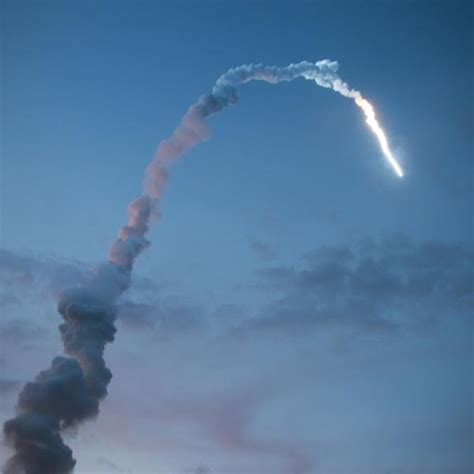
\includegraphics[width=60mm]{A2022.IDSEPC.ProcessoDiProduzione/Ariane5.jpeg}
\end{center}

\end{frame}



\begin{frame}{\centerline{Software Engineering (1/2)}}
% Nr:1
\begin{center}
Software Engineering o Ingegneria del Software\\
\vspace{1cm}
{\Large
Ingegnerizzare la produzione del software\\
}
\vspace{2cm}
Spesso si fanno analogie tra la produzione del software e cucinare...
\end{center}
\end{frame}

\begin{frame}{\centerline{Software Engineering (2/2)}}
% Nr:1
\begin{center}
\Large
Che lo show abbia inizio!\\
\vspace*{0.5cm}
Signore e signori: \textcolor{red}{Charlie Chaplin}
\end{center}
\begin{center}
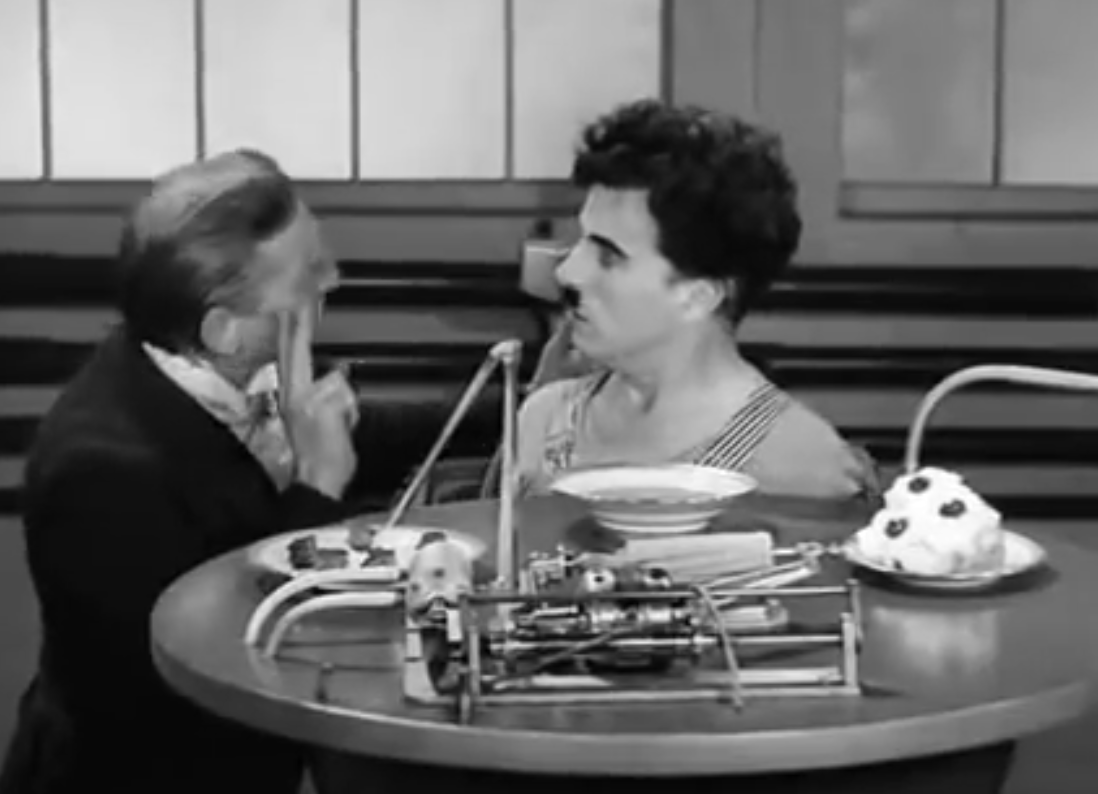
\includegraphics[width=60mm]{A2022.IDSEPC.ProcessoDiProduzione/Chaplin_ModernTimes.png}
\end{center}

\end{frame}



\begin{frame}{\centerline{Sondaggio}}
\begin{center}
Sulla base del video, qual \`{e} lo scopo dell'ingegneria dle software?
\end{center}
\end{frame}

\begin{frame}{\centerline{Idee}}
\noindent\makebox[\linewidth]{\rule{\paperwidth}{0.4pt}}\\
\vspace{0.5cm}

\noindent\makebox[\linewidth]{\rule{\paperwidth}{0.4pt}}\\
\vspace{0.5cm}

\noindent\makebox[\linewidth]{\rule{\paperwidth}{0.4pt}}\\
\vspace{0.5cm}

\noindent\makebox[\linewidth]{\rule{\paperwidth}{0.4pt}}\\
\vspace{0.5cm}

\noindent\makebox[\linewidth]{\rule{\paperwidth}{0.4pt}}\\
\vspace{0.5cm}

\noindent\makebox[\linewidth]{\rule{\paperwidth}{0.4pt}}\\
\vspace{0.5cm}

\noindent\makebox[\linewidth]{\rule{\paperwidth}{0.4pt}}\\

\end{frame}

\begin{frame}{\centerline{La mia idea dell'ingegnere del software}}

\begin{center}
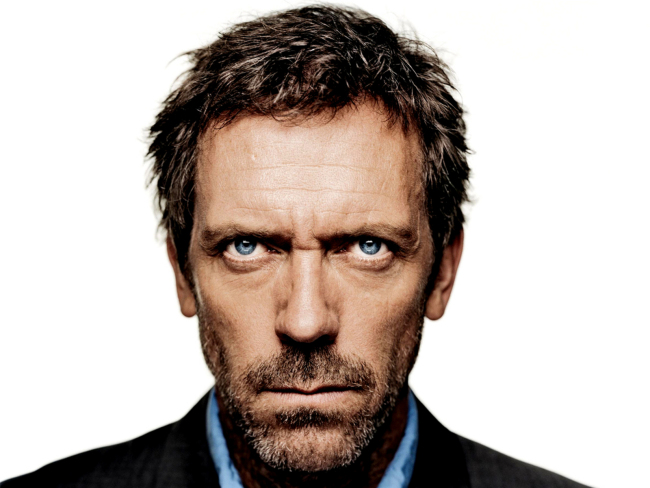
\includegraphics[width=80mm]{A2022.IDSEPC.ProcessoDiProduzione/DrHouse_SoftwareEngineer.jpg}
\end{center}

\end{frame}

\begin{frame}{\centerline{Continuiamo lo show!}}
\vspace*{1.5cm}
\begin{center}
\Huge Video on Dr. House

\end{center}

\end{frame}

\begin{frame}{\centerline{Lean Software Development}}
Lean software development o approccio lean alla produzione del software\\
\vspace{1cm}
\begin{center}
Lean software development o approccio lean alla produzione del software\\
\vspace{1cm}
\LARGE
Premesse sul Lean Management
\end{center}
\end{frame}

\begin{frame}{\centerline{La ``Software Crisis'' (1/3)}}
% Nr:2
La ``Software Crisis'' o ``crisi del software'' \`{e} il fenomeno dovuto all'aumento della potenza dei calcolatori: in termini \textit{terra terra}, finch\'{e} i calcolatori erano molto piccoli, la programmazione non presentava problemi, quando le macchine hanno iniziate a crescere, i problemi hanno iniziato a comparire, e ora che abbiamo computer giganteschi, la programmazione è pure diventata un problema gigantesco.\\
Edsger Dijkstra, \textcolor{red}{\bf 1972}
\begin{center}
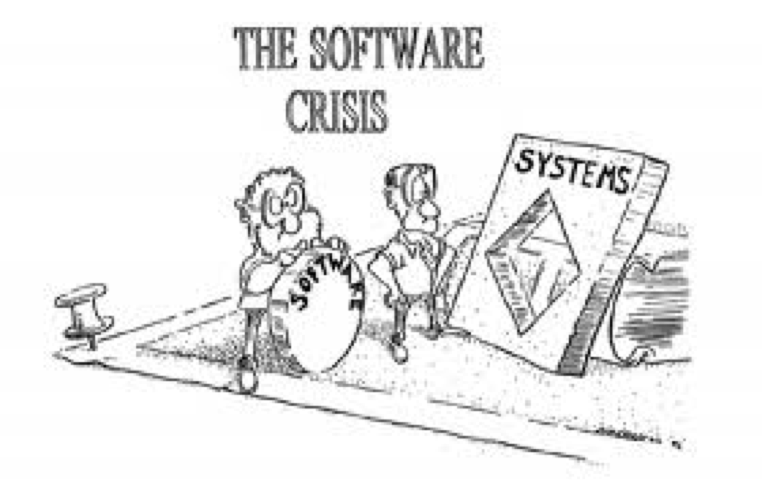
\includegraphics[width=55mm]{A2022.IDSEPC.ProcessoDiProduzione/pic-01.png}
\end{center}



\begin{center}
\tiny
\url{http://qualityandprogramming.blogspot.ru/2012/03/crisis-del-software.html}
\end{center}

\end{frame}

\begin{frame}{\centerline{La ``Software Crisis'' (2/3)}}
% Nr:3
Sequenze di rivoluzioni tecnologiche si sono viste in molte aree dello scibile umano grazie al software.

\begin{center}
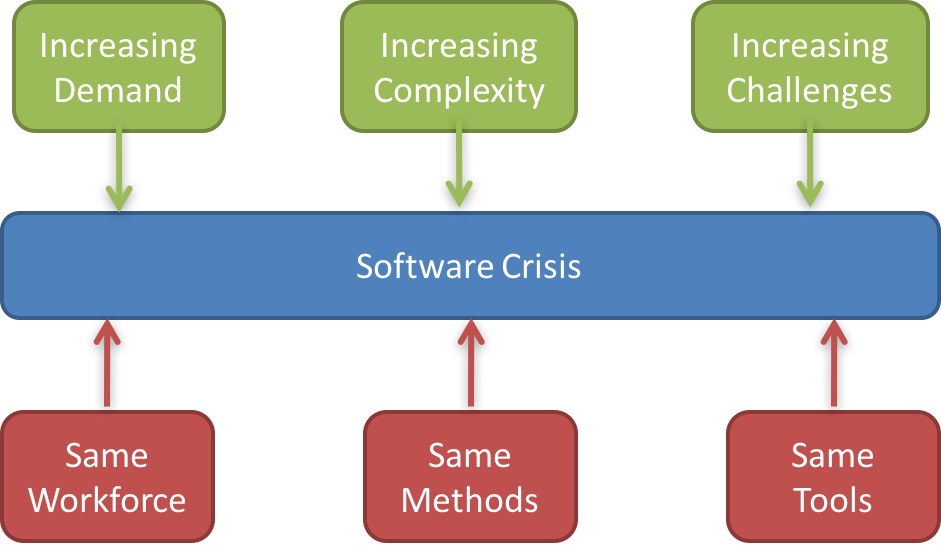
\includegraphics[width=80mm]{A2022.IDSEPC.ProcessoDiProduzione/pic-02.png}
\end{center}
Purtroppo, l'ingegneria del software non ha avuto una analoga rivoluzione!

\begin{center}
\tiny
\url{http://www.slideshare.net/rui\_curado/abse-and-atomweaver-a-quantum-leap-in-software-development}
\end{center}



\end{frame}
\begin{frame}{\centerline{La ``Software Crisis'' (3/3)}}
% Nr:4
Le cause della crisi del software sono collegate  alla complessit\`{a} crescente di hardware e software associato, e tale crisi si \`{e} manifestata in una moltitudine di modi:
\begin{itemize}
\item Progetti che sforano il budget
\item Progetti che non rispettano i tempi
\item Sistemi software inefficienti
\item Sistemi software di bassa qualit\`{a}
\item Sistemi software che non rispndono a requisiti
\item Progetti diventati ingestibili
\item Codice software illeggibile e impossibile da mantenere
\item Software mai consegnato al cliente
\end{itemize}

\begin{small}
https://en.wikipedia.org/wiki/Software\_crisis
\end{small}
\end{frame}

\begin{frame}{\centerline{Esempi di errori dei sistemi software (1/2)}}


\textbf{NASA’s Mars Climate Orbiter} -- Nella rotta verso Marte nel 1998 il Climate Orbiter spacecraft si `\`{e} perso nello spazio. Anche se inizialmente non si cap\`{i} la ragione dell'errore, alla fine si trov\`{o} che un subcontraente commise un banale errore di trasformazioni delle misure dal sistema inglese a quello metrico.
\vspace{0.5cm}

Questa svista imbarazzante sped\`{i} la navetta spaziale da 
 \textcolor{red}{\bf 125 milioni di dollari} fatalmente vicina alla superficie di Marte dopo aver tentato di stabilizzare la sua orbita troppo in basso.
\newline 
\vspace{1cm}
\begin{center}
    \tiny
    Estratto con modifiche da:
\url{https://raygun.com/blog/2014/05/10-costly-software-errors-history/}
\end{center}
\end{frame}

\begin{frame}{\centerline{Esempi di errori dei sistemi software (2/2)}}
\small
\textbf{Ariane 5 Flight 501} -- L'allora nuovissimo satellite europeo riutilizz\`{o} un software dal suo predecessore, l'Ariane 4. Sfortunatamente, l'Ariane 5 aveva un motore pi\`{u} veloce e questo rivel\`{o} un baco precedentemente passato inosservato. Dopo 36 secondi dal lancio, i progettisti inziarono l'operazione di autodistruzione a seguito di una serie di errori dei computer. In sintesi, il software stava provando a inserire un numero a 64 bit in uno spazio di 16 bit, con il risultato di mandare in tilt sia i computer primari che quelli ausiliari, visto che entrambi usavano lo stesso software.
\vspace{0.5cm}

La costruzione dell'Ariane 5 era costata \textcolor{red}{\bf 8 billioni di dollari}  e stava trasportando un satellite da \textcolor{red}{\bf 500 millioni di dollari}. 
\newline 
\vspace{1cm}
\begin{center}
    \tiny
    Estratto con modifiche da: \url{https://raygun.com/blog/2014/05/10-costly-software-errors-history/} Video:  \url{https://youtu.be/qnHn8W1Em6E}
\end{center}

\end{frame}

\begin{frame}{\centerline{Ancora sulla ``Software Crisis'' (1/2)}}
% Nr:5
Le problematicit\`{a} nello sviluppo software proviene dalla nostra intrinsica limitazione nel comprenderlo, e dalle difficolt\`{a} strutturali, che possono essere divise in quattro categorie:
\begin{itemize}
\item \textcolor{red}{\bf Complessit\`{a}:} i sistemi software consistono di parti multiple e diverse che possono essere in molti stati diversi. Questo li rende difficile ad essere concepiti, descritti e controllati.

\item \textcolor{red}{\bf Conformit\`{a}:} molto spesso il software deve essere integrato con altro software sviluppato precedentemente in contesti e con regolamentazioni che possono essere diverse. Tutti queste condizioni e vincoli crescono ed evolvono nel tempo e rendono anche molto probabile che il software debba essere cambiato in futuro.
%Succi.B7 c1.1. p.7 
\end{itemize}

\end{frame}

\begin{frame}{\centerline{Ancora sulla ``Software Crisis'' (2/2)}}
% Nr:6
\begin{itemize}
\item \textcolor{red}{\bf Changeability:} all successful software gets changed - as new uses of a software product are found, stakeholders push for modifications. Moreover, successful software survives the life cycle of the environment (e.g., operating system, hardware, etc.) it was written for. This means software has to be updated to the new needs or environments it has to run it;

\item \textcolor{red}{\bf Invisibility:} the invisibility of software and the difficulties in visualizing it make it difficult to reason and to communicate about it.
%Succi.B7 c1.1. p.7
\end{itemize}
\end{frame}

\begin{frame}{\centerline{Understanding better the nature of software}}
% Nr:7
\begin{itemize}
\item If software is not tangible concretely, perhaps it can be viewed as a creative art
\item Software is about writing, so, let's turn our attention to writing
\item Assignment: 
\begin{itemize}
\item preparation of a 5 minutes and 5 slides presentation for next class based on the book: ``Six Memos for the Next Millennium'' by Italo Calvino
\item the groups are as for the report
\item the specific chapter assigned to each group is defined in the workbook
\item there is a LaTeX template already ready in overleaf
\item you should focus on two aspects:
\begin{enumerate}
\item what you find in the chapter already present in software,
\item what you find in the chapter that should be present in software but right now it is not.
\end{enumerate}
\item deadline for the slides: January 28th 2020 at midnight.
\end{itemize}
\end{itemize}

\end{frame}



%====================================================================================

\begin{frame}{\centerline{Tame and Wicked Problems}}
% Nr:7
\begin{small}
\textbf{Tame problems} are those problems that can be easy engineered; they can be formulated exhaustively and stated containing all the information needed for understanding and solving the problem.

Not all problems are tame. There are also \textbf{wicked problems}. The information needed to describe the wicked problem depends on the idea to solve it.

\begin{center}
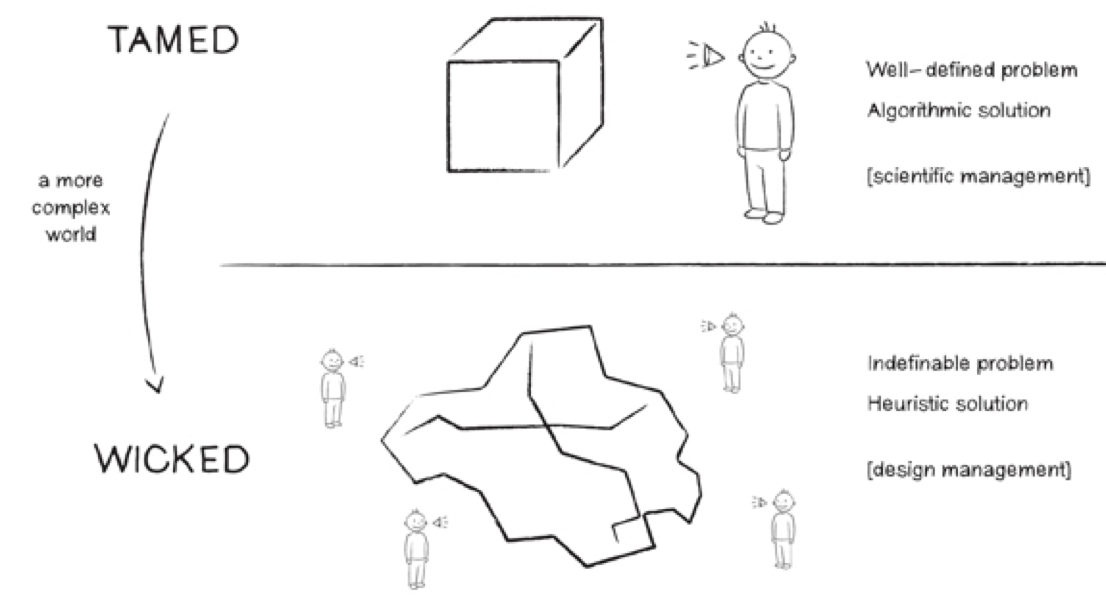
\includegraphics[width=70mm]{A2022.IDSEPC.ProcessoDiProduzione/pic-03.png}
\end{center}

\end{small}

\begin{center}
\tiny
\url{https://vivifychangecatalyst.wordpress.com/2015/06/28/wicked-problems-innovation-and-project-masiluleke}

\end{center}


\end{frame}

%====================================================================================

\begin{frame}{\centerline{Tame Problems}}
% Nr:8
\begin{itemize}
\item Has a well-defined and stable problem statement.
\item Has a definite stopping point, i.e., when the solution is reached.
\item Has a solution which can be objectively evaluated as right or wrong.
\item Belongs to a class of similar problems which are all solved in the same similar way.
\item Has solutions which can be easily tried and abandoned.
\item Comes with a limited set of alternative solutions
\end{itemize}
%Succi.B7 c1.2. p.9
\begin{center}
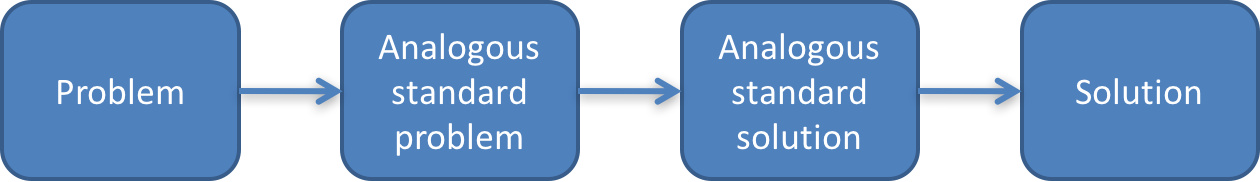
\includegraphics[width=80mm]{A2022.IDSEPC.ProcessoDiProduzione/pic-04.png}
\end{center}

\begin{center}
\tiny
\url{http://www.slideshare.net/curtistim/wicked-issues-taming-problems-and-systems}
\end{center}

\end{frame}

%====================================================================================

\begin{frame}{\centerline{Wicked Problems}}
% Nr:9
\small
\begin{itemize}
\item Wicked projects cannot provide a definitive, analytical formulation of the problem they target. Formulating the project and the solution is essentially the same task. Each time you attempt to create a solution, you get a new, hopefully better, understanding of the project.

\item Wicked projects have no a stopping rule telling when the problem they target has been solved. The problem-solving process proceeds iteratively and ends when resources are depleted and/or stakeholders lose interest in a further refinement of the currently proposed solution.

\item Solutions to problems in wicked projects are not true or false, but good or bad. Since there are no unambiguous criteria for deciding if the project is resolved, getting all stakeholders to agree that a resolution is ``good enough'' can be a challenge.
\end{itemize}
%Succi.B7 c1.2. p.9

\end{frame}

%====================================================================================

\begin{frame}{\centerline{Wicked Problems}}
% Nr:10
\small
\begin{itemize}
\item There is no immediate or ultimate test of a solution to the targeted problem in a wicked project. Solutions to such projects generate waves of consequences, and it is impossible to know how these waves will eventually play out.

\item Each solution to the problem targeted by a wicked project has irreversible consequences. Care must be placed in managing assumed solutions. Once the website is published or the new customer service package goes live, you cannot take back what was online or revert to the former customer database.

\item Wicked projects do not have a well-described, widely accepted set of potential solutions. The various stakeholders may have differing views of what are acceptable solutions. It is a matter of judgment as to when enough potential solutions have emerged and which should be pursued.

\end{itemize}
%Succi.B7 c1.2. p.9

\end{frame}
\begin{frame}{\centerline{Wicked Problems}}
% Nr:11
\small
\begin{itemize}
\item Each wicked project is essentially unique. There are no well-defined ``classes'' of solutions that can be applied to a specific case. It is not easy to find analogous projects, previously solved and well documented, so that their solution could be duplicated.

\item The problem targeted by a wicked project can be considered a symptom of another problem. A wicked project deals with a set of interlocking issues and constraints that change over time, embedded in a dynamic and evolving context.

\item The causes of a problem targeted by a wicked project can be explained in several ways. There are several stakeholders who have various and changing ideas about what is the project, its nature, its causes, and the associated solution.

\item The project must not go wrong. Mistake is not an option here. Despite the inability to express the project solution analytically, it is not allowed to fail the project.
\end{itemize}
%Succi.B7 c1.2. p.9

\end{frame}
\begin{frame}{\centerline{Software Development Is a Wicked Problem}}
% Nr:12
\small
\begin{itemize}
\item It is very hard to plan a software development project upfront considering all eventualities.

\item A software product is hardly perfect or finished; as soon as users use it, new requirements will arise.

\item There does not exist the one single solution to a software engineering problem.

\item We cannot determine how well an implementation solves the requirements until we implement it.

\item Choices are sometimes very costly to reverse. The last option is to throw away the existing product and start from scratch.

\end{itemize}
%Succi.B7 c1.3. p.10

\end{frame}
\begin{frame}{\centerline{Software Development Is a Wicked Problem}}
% Nr:13
\small 
\begin{itemize}
\item There are infinite ways to solve a software development problem.

\item Every software development project is essentially unique.

\item Software engineering is a wicked problem on multiple levels: choosing the ``best'' database system, user interface, operating system, hardware, etc. is also a wicked problem.

\item The problem a software system aims to solve is seen differently by the stakeholders of the system: users, developers, maintainers, database operators, etc.

\item Software development (i.e., to try to solve the problem) means to spend resources. To be wrong, i.e., to deliver a solution that the users retain not useful, is not considered an option.

\end{itemize}
%Succi.B7 c1.3. p.10

\end{frame}

%---------------------------------------------
\begin{frame}{\centerline{Keeping the Process Under Control}}
% Nr:14

Michael L. Harris proposed an effective way to classify different types of control and in which circumstances these types work best.
\newline 

The selection of the most effective control mechanism depends on two factors:
\begin{itemize}
\item  the ability to measure the output, the ``measurability,'' and

\item  the ability to specify in details the steps required to accomplish a given task, the ``specifiability.''
\end{itemize}
\end{frame}
%=============================================

%---------------------------------------------
\begin{frame}{\centerline{Keeping the Process Under Control}}
% Nr:15
So if we put these two factors in a two-dimensional diagram, we obtain four areas:
\begin{itemize}


\item  an area with high level of measurability and of specifiability;

\item  an area where we have a high level of measurability of the output but little specifiability;

\item  an area where we have a high level of specifiability but little measurability; and

\item  an area where we can neither measure directly the output nor specify the steps of the work.
\end{itemize}
\end{frame}
%=============================================

%---------------------------------------------
\begin{frame}{\centerline{Keeping the Process Under Control}}
% Nr:16

\begin{center}
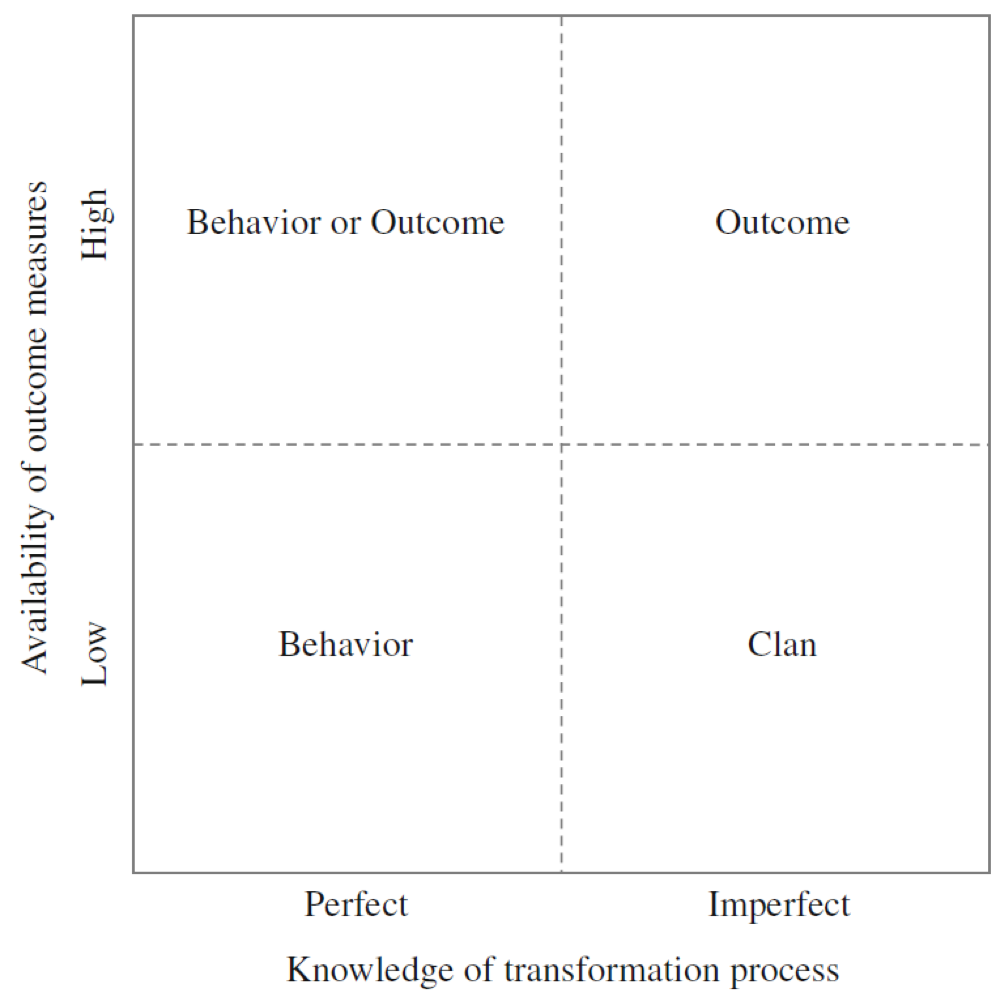
\includegraphics[width=70mm]{A2022.IDSEPC.ProcessoDiProduzione/img-img03.png}
\end{center}
\end{frame}
%=============================================

\begin{frame}{\centerline{Coordination mechanisms}}
% Nr:57
\begin{center}

\includegraphics[width=20mm]{A2022.IDSEPC.ProcessoDiProduzione/img-img10.png}
\end{center}

According to Malone and Crowston (1994) there are three ways people coordinate:
\begin{itemize}
\item  Sequentially or individual
\item  Via shared resource
\item  Via common output
\end{itemize}

\end{frame}
%=============================================

%---------------------------------------------
\begin{frame}{\centerline{Sequential}}
% Nr:58

\begin{center}
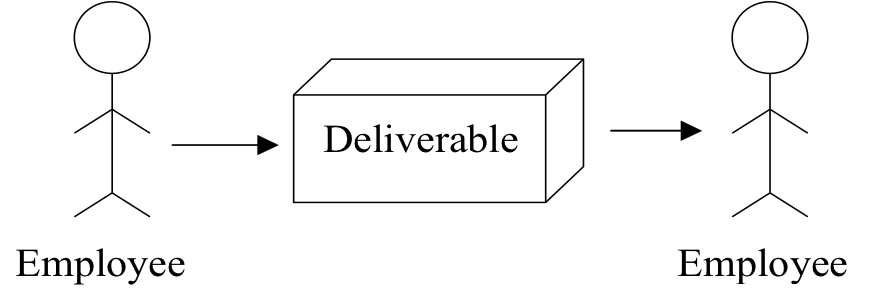
\includegraphics[width=70mm]{A2022.IDSEPC.ProcessoDiProduzione/img-img11.png}
\end{center}

\begin{itemize}
\item  First write the analysis document


\item  On the basis of the analysis document write the design document


 
\end{itemize}

(Is this endogenous control?)
\end{frame}
%=============================================

%---------------------------------------------
\begin{frame}{\centerline{Shared resource}}
% Nr:59
\begin{center}
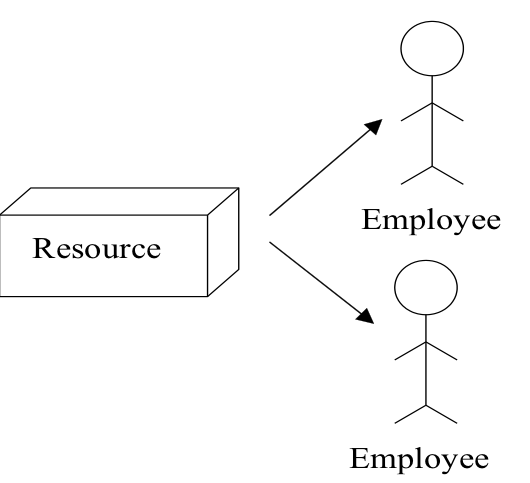
\includegraphics[width=50mm]{A2022.IDSEPC.ProcessoDiProduzione/img-img12.png}
\end{center}

\begin{itemize}
\item  The development may start only after the customer has committed to the project

\item  The classes to develop are assigned to developers on a \\ First Come – First Served basis

\end{itemize}


\end{frame}
%=============================================

%---------------------------------------------
\begin{frame}{\centerline{Common output}}
% Nr:60
\begin{center}
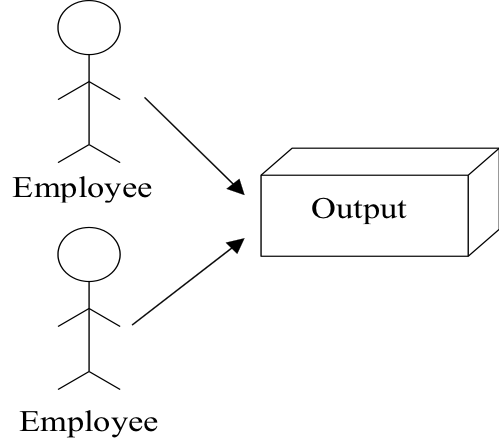
\includegraphics[width=50mm]{A2022.IDSEPC.ProcessoDiProduzione/img-img13.png}
\end{center}

\begin{itemize}
\item  The team leader proposes a schedule for the week to come; the team has to agree unanimously on it

\item  The team sits together to produce the final release that requires everyone approval
  
\end{itemize}


\end{frame}
%=============================================

%---------------------------------------------
\begin{frame}{\centerline{What is most difficult?}}
% Nr:61
\begin{itemize}

\item  Easiest: Sequential
\item  Then: Shared resource -- there is the need to respect priorities
\item  Most difficult: Common output
\begin{itemize}

\item  people need to work together, hand in hand, producing the same good
\end{itemize}

\item Most of traditional software development is based on exogenous control and sequential coordination 

\end{itemize}

\end{frame}
%=============================================


%---------------------------------------------
\begin{frame}{\centerline{Agile Manifesto}}
% Nr:3
\begin{center}
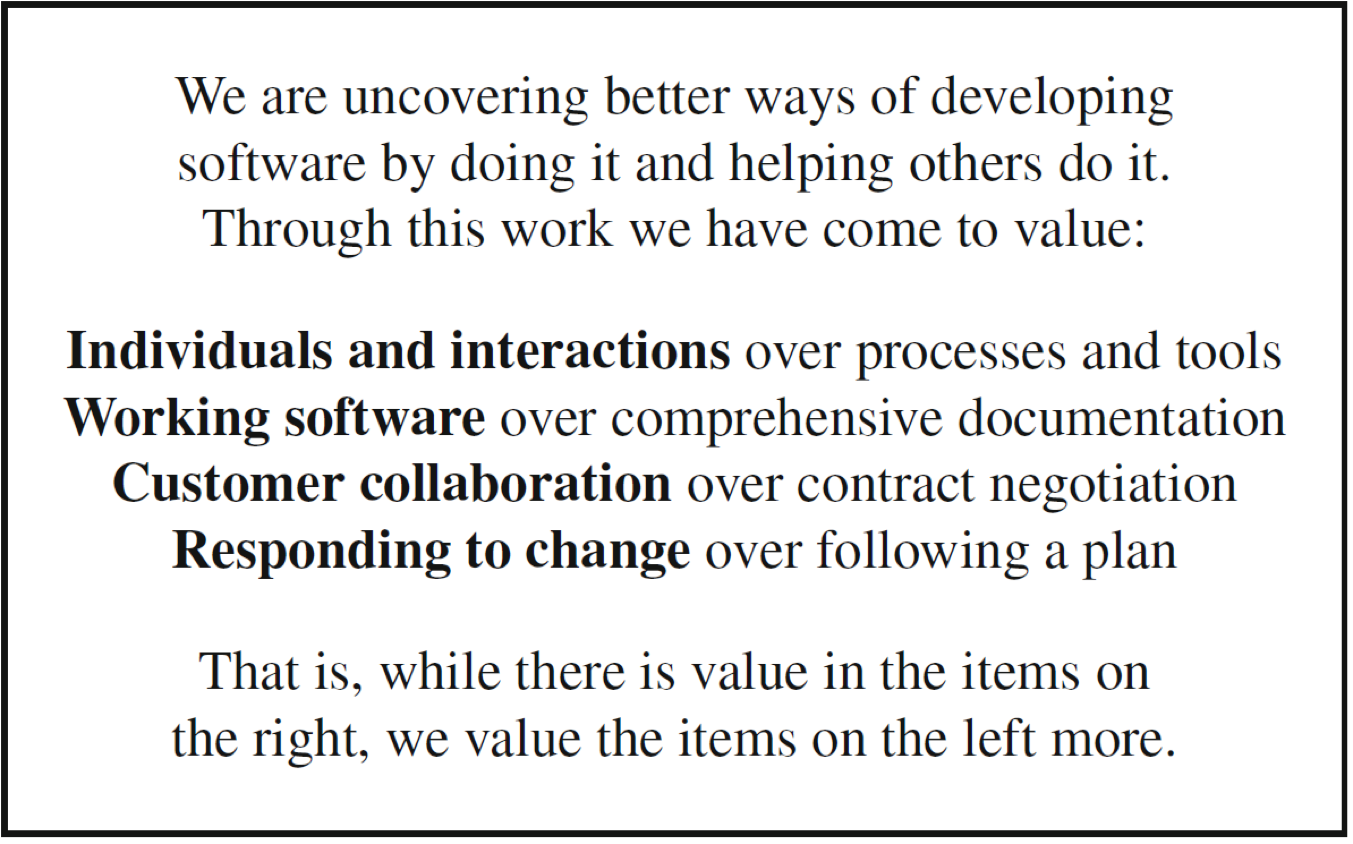
\includegraphics[width=90mm]{A2022.IDSEPC.ProcessoDiProduzione/img-img00.png}
\end{center}
\end{frame}
%=============================================

\begin{frame}{\centerline{Waterfall development model}}
% Nr:8

The waterfall model was the first to address risks, namely it focused on the \textcolor{red}{to develop a product that does not correspond to the requirements}.\\

To handle such risk properly, the design was done only after the requirements were clear, the implementation was done after the design was completed, the system was then verified and tested at the end to again ensure that it did what it should do.


\footnotetext[1]{\url{http://www.railshorde.com/blog/waterfall-development-model}}
\end{frame}

\begin{frame}{\centerline{Waterfall development model -- Schema}}
% Nr:8

\begin{center}
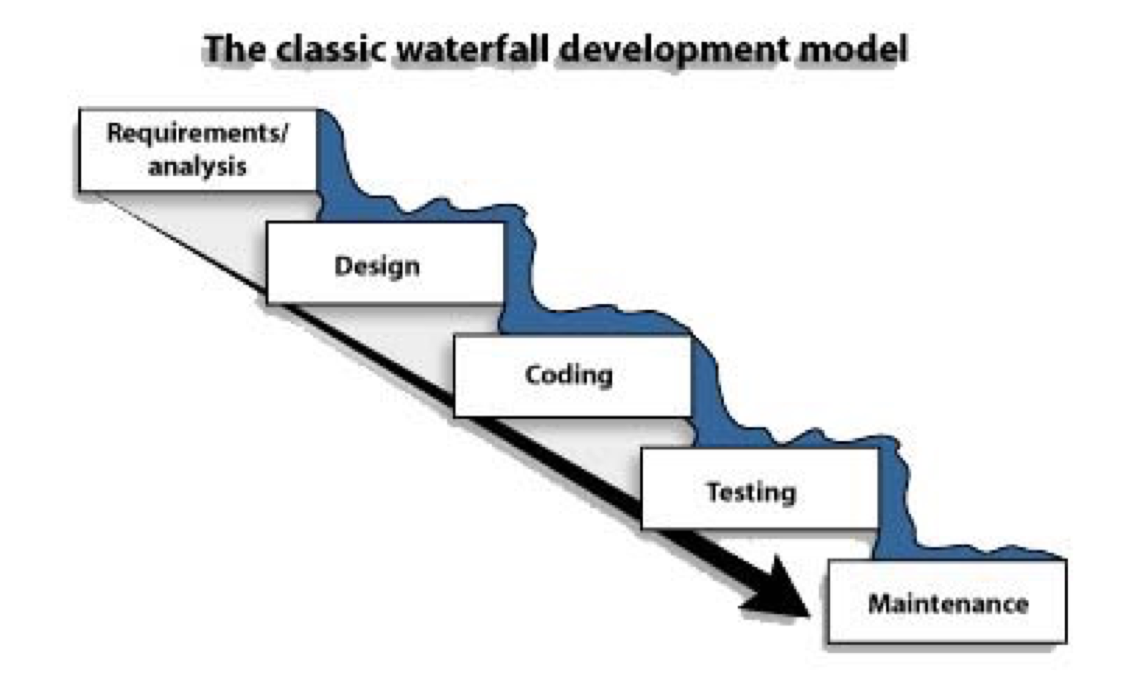
\includegraphics[width=90mm]{A2022.IDSEPC.ProcessoDiProduzione/img-02.png}
\end{center}
\small
\footnotetext[1]{\url{http://www.railshorde.com/blog/waterfall-development-model}}
\end{frame}

\begin{frame}{\centerline{Waterfall development model}}
% Nr:9
The phases in Waterfall model are discussed in detail as follow:
\newline

\textbf{Planning and Requirements:} All possible requirements of the system to be developed are gathered in this phase and planning for further development is done in advance to produce a Quality product within the given time and cost.
\newline

\textbf{Analysis and System Design:} The requirements captured in first phase are deeply analyzed and then a system design is prepared. This system design is the blue print of the system to be developed. System Design helps in defining hardware and software needs of the system and also specifies the overall system architecture.
\newline

\footnotetext[1]{\url{http://www.railshorde.com/blog/waterfall-development-model}}
\end{frame}

\begin{frame}

\textbf{Construction and Modeling:} With the inputs of previous phase the actual coding is done in this phase to develop the system. The developer is responsible for the coding part. The system is first developed in small programs called units, which are integrated in the next phase.
\newline

\textbf{Integration and Testing:} All the individual units developed in the Construction phase are integrated into a system as a whole after each unit is tested thoroughly called as Unit testing. Then the whole system all together is tested for any faults or defects.
\newline

\footnotetext[1]{\url{http://www.railshorde.com/blog/waterfall-development-model}}
\end{frame}

\begin{frame}{\centerline{Waterfall development model}}
% Nr:10


\textbf{Deployment of system:} After the Unit and System testing is done and all the bugs are resolved, the product is deployed to the customer.
\newline

\textbf{Maintenance:} There are some issues which are encountered by the client or the customer after deployment, fixing of those issues comes under Maintenance phase. Also to enhance the product some better versions are released. Maintenance is done to deliver these changes in the customer environment.
\newline

\footnotetext[1]{\url{http://www.railshorde.com/blog/waterfall-development-model}}
\end{frame}
\begin{frame}{\centerline{Waterfall development model}}
% Nr:11

\textbf{Advantages of Waterfall Model:}
\begin{itemize}
\item  Simple and easy to use and understand.

\item  Each phase is processed one at a time, so full dedication is on one process only.

\item  Works well for smaller projects where requirements are well understood.

\item  Each stage has its own task to do deliberately.

\item  Each process is fully documented to avoid further difficulties.

\end{itemize}

\footnotetext[1]{\url{http://www.railshorde.com/blog/waterfall-development-model}}
\end{frame}
\begin{frame}{\centerline{Waterfall development model}}
% Nr:12

\textbf{Disadvantages of Waterfall Model:}
\begin{itemize}
\item  The biggest problem arises that no another process can come under work simultaneously.

\item  The requirements are to be predefined at the initial stage; if requirements are identified at later stage of time then they cannot be easily appended at the existing Waterfall Cycle.

\item  Waterfall Model does not allow iterations of phases. The whole project can be integrated at the end only.

\item  The customers can preview project at end only. No earlier prototype is released and shown to user.
\end{itemize}


\footnotetext[1]{\url{http://www.railshorde.com/blog/waterfall-development-model}}
\end{frame}
\begin{frame}{\centerline{Waterfall development model}}
% Nr:13

\textbf{Applications of Waterfall Model:}
\begin{itemize}

\item  There are no ambiguous requirements.

\item  Requirements are very well documented and fixed beforehand.

\item  Technology is not dynamic.

\item  Product definition is stable.

\item  Sufficient resources and expertise are available to support the product.
\end{itemize}

\footnotetext[1]{\url{http://www.railshorde.com/blog/waterfall-development-model}}
\end{frame}
\begin{frame}{\centerline{Spiral development model}}
% Nr:14
\begin{center}
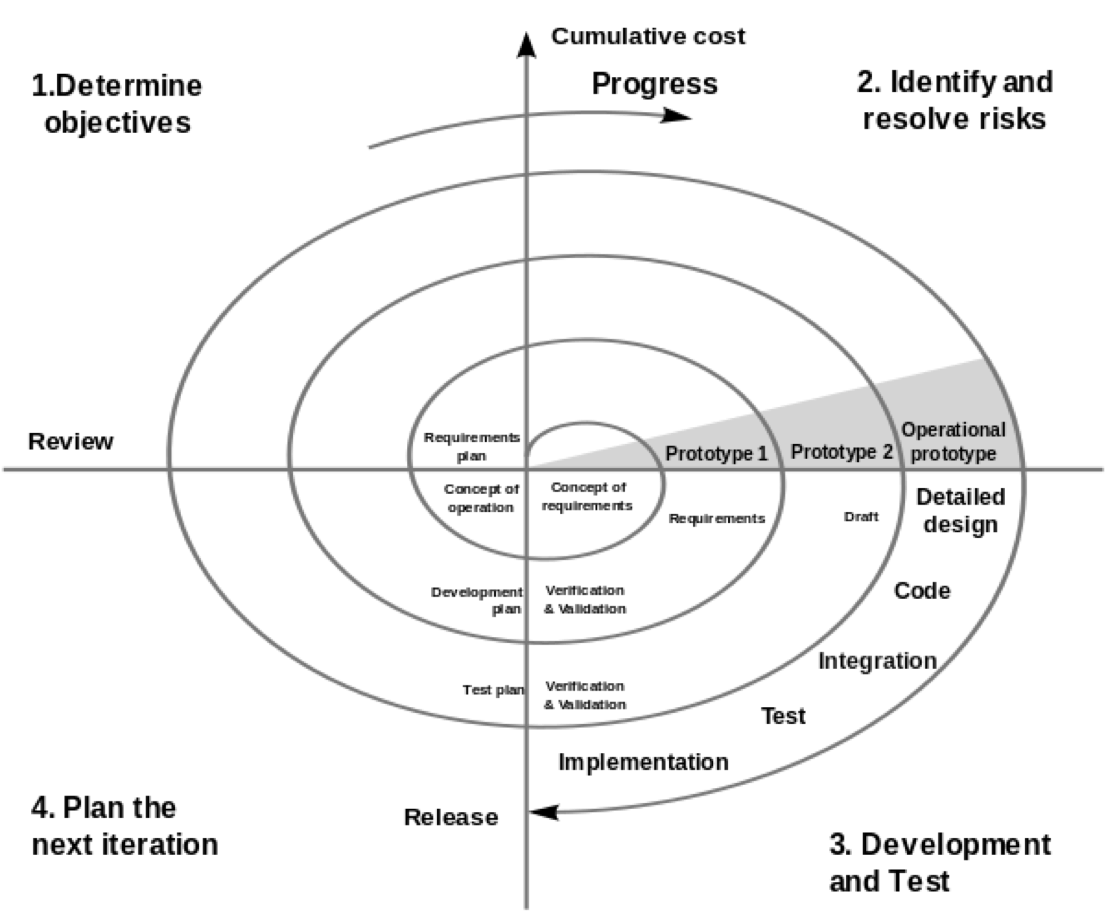
\includegraphics[width=80mm]{A2022.IDSEPC.ProcessoDiProduzione/img-03.png}
\end{center}


\footnotetext[1]{\url{https://en.wikipedia.org/wiki/Spiral\_model}}
\end{frame}
\begin{frame}{\centerline{Spiral development model}}
% Nr:15

The spiral software development model is an iterative software development approach in which each cycle shows the following characteristics:

\begin{itemize}


\item  Concurrent rather than sequential determination of artifacts.

\item  Consideration in each spiral cycle of the main spiral elements:

\begin{itemize}
\item  critical stakeholder objectives and constraints,

\item  product and process alternatives,

\item  risk identification and resolution,

\item  stakeholder review,

\item  commitment to proceed.
\end{itemize}
\end{itemize}
\end{frame}
\begin{frame}{\centerline{Spiral development model}}
% Nr:16

\begin{itemize}
\item  Using risk considerations to determine the level of effort to be devoted to each activity within each spiral cycle.

\item  Managing stakeholder life cycle commitments.

\item  Emphasis on activities and artifacts for system and life cycle rather than for software and initial development.

\end{itemize}


\end{frame}


%---------------------------------------------
\begin{frame}{\centerline{Agile Manifesto}}
% Nr:4

The ``Agile Manifesto'' identifies two sets of values: the values lying on the left of the document and the values lying on the right of the document.
\begin{center}
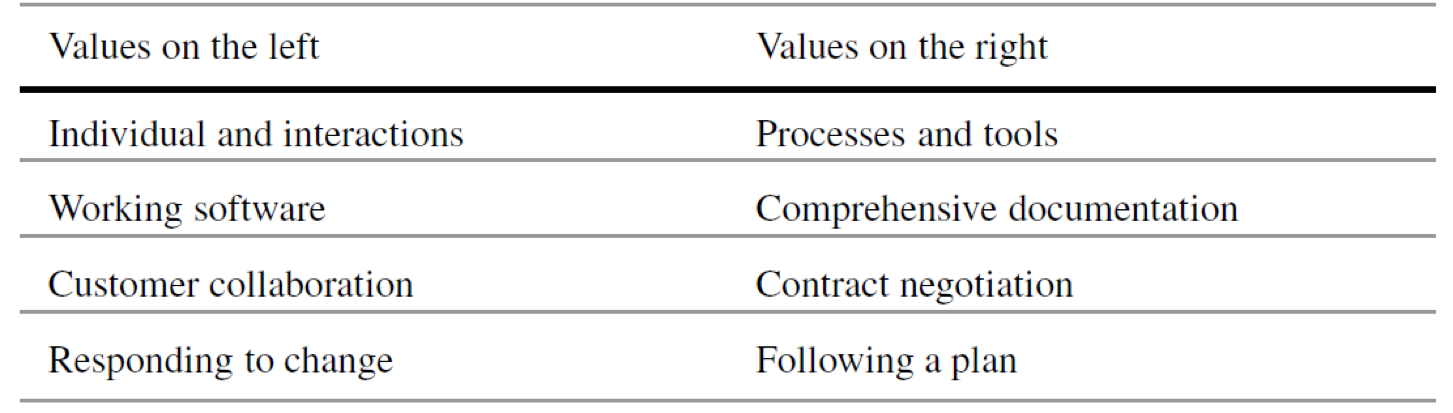
\includegraphics[width=120mm]{A2022.IDSEPC.ProcessoDiProduzione/img-img01.png}
\end{center}
\end{frame}
%=============================================

%---------------------------------------------
\begin{frame}{\centerline{Agile Manifesto I}}
% Nr:5
\begin{itemize}
\item  Our highest priority is to satisfy the customer through early and continuous delivery of valuable software

\item  Welcome changing requirements, even late in development, Agile processes harness change for the customer's advantage

\item  Business people and developers must work together daily throughout the project

\end{itemize}
\end{frame}
%=============================================

%---------------------------------------------
\begin{frame}{\centerline{Agile Manifesto II}}
% Nr:6
\begin{itemize}
\item  Deliver working software frequently, from a couple of weeks to a couple of months, with a preference to the shorter timescale

\item  Build projects around motivated individuals

\item  Give them the environment and support they need, and trust them to get the job done

\end{itemize}
\end{frame}
%=============================================

%---------------------------------------------
\begin{frame}{\centerline{Agile Manifesto III}}
% Nr:7
\begin{itemize}
\item  The most efficient and effective method of conveying information to and within a development team is face-to-face conversation

\item  Working software is the primary measure of progress

\end{itemize}
\end{frame}
%=============================================

%---------------------------------------------
\begin{frame}{\centerline{Agile Manifesto IV}}
% Nr:8
\begin{itemize}
\item  Agile processes promote sustainable development. The sponsors, developers, and users should be able to maintain a constant pace indefinitely

\item  Continuous attention to technical excellence and good design enhances agility
(continued)
\end{itemize}
\end{frame}
%=============================================

%---------------------------------------------
\begin{frame}{\centerline{Agile Manifesto V}}
% Nr:9
\begin{itemize}
\item  Simplicity -- the art of maximizing the amount of work not done -- is essential

\item  The best architectures, requirements, and designs emerge from self-organizing teams

\item  At regular intervals, the team reflects on how to become more effective, then tunes and adjusts its behavior accordingly
\end{itemize}
\end{frame}
%=============================================




\begin{frame}
{\centerline{Questions?}}
\vspace{1cm}
\begin{center}
    \LARGE{End of the fifth lecture.}
\end{center}

\end{frame}

\end{document}


